%Dokumentacja techniczna projektu Rękawica Sensoryczna 2017
\usepackage{graphicx}
\usepackage{hyperref}


\renewcommand{\maketitle}{\begin{titlepage}

\begin{center}


\LARGE\centering Dokumentacja techniczna projektu Rękawica Sensoryczna\\
\large\centering Projekt realizowany w ramach kursu Roboty Mobilne 1 na Politechnice Wrocławskiej\\
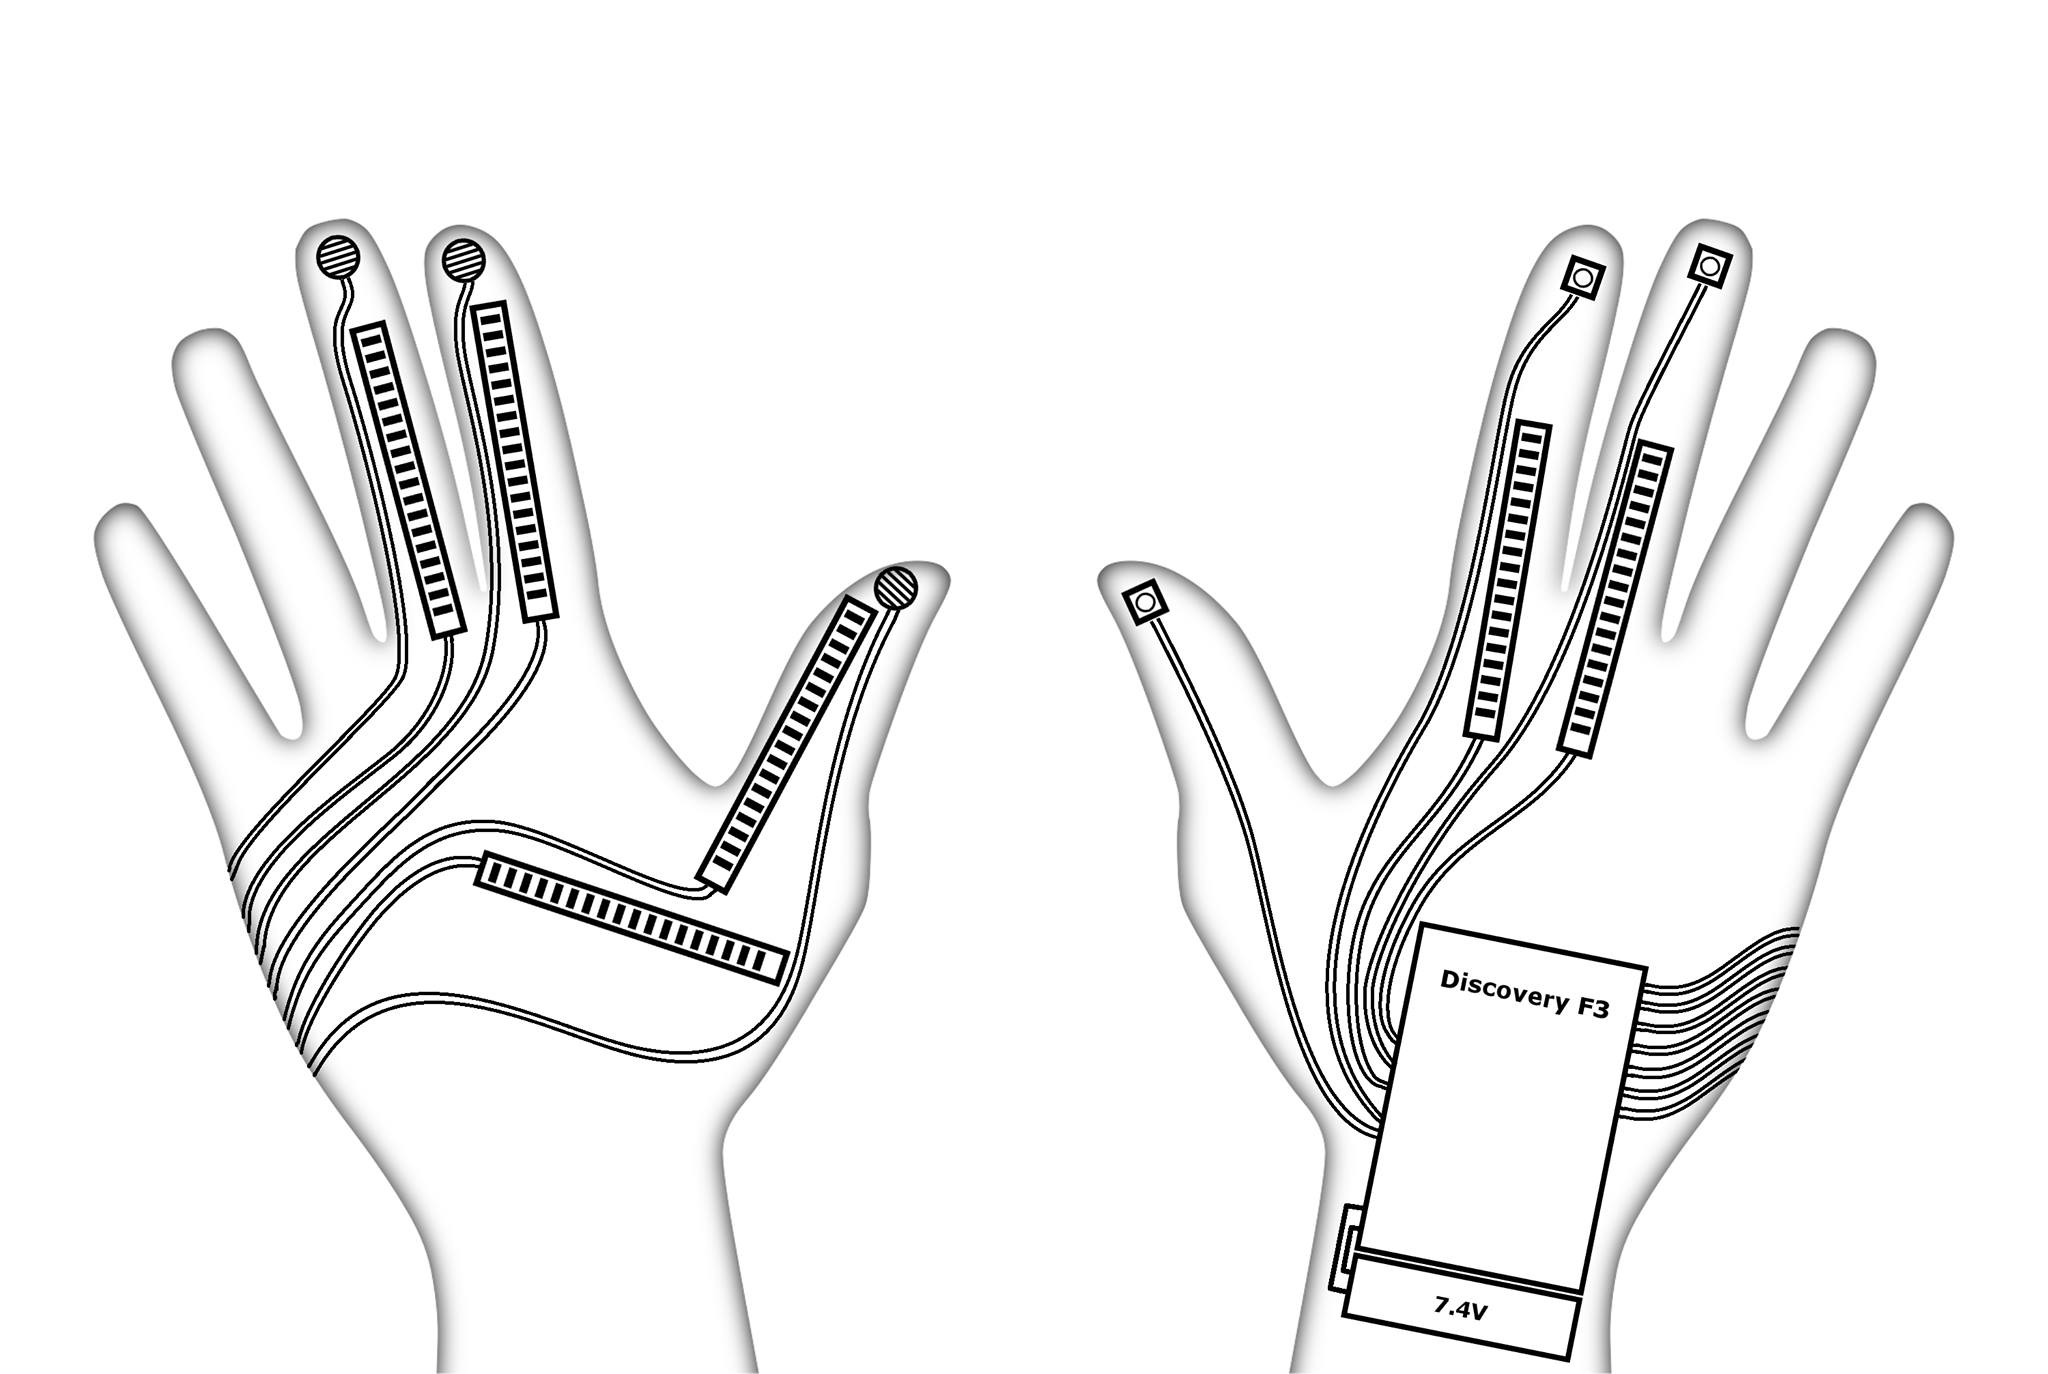
\includegraphics[width=0.7\textwidth]{images/rekawica_old.jpg}
\vspace*{2cm}
\normalsize\flushleft\textbf{Temat Projektu:} Rękawica sensoryczna\\
\textbf{Autorzy:} Krzysztof Dąbek 218549, Dymitr Choroszczak 218627,\\Anna Postawka 218556\\
\textbf{Kierunek:} Automatyka i Robotyka\\
\textbf{Specjalność:} Robotyka (ARR)\\
\textbf{Prowadzący:} dr inż. Andrzej Wołczowski\\
\textbf{Kurs:} Roboty Mobilne 1\\
\textbf{Termin zajęć:} pn TN 11:15, śr TN 14:30\\
\vspace{5 mm}



\vspace*{3.5cm}
\centering\textsc{\today}\\

\end{center}
\end{titlepage}
\newpage
}